\documentclass{beamer} 

\usepackage[utf8]{inputenc}
\usepackage[T1]{fontenc}
\usepackage{graphicx}
\usepackage[serbian]{babel}
\usepackage{multicol}
\usepackage{tikz}
\usetikzlibrary{shapes.geometric, arrows}


\usetheme{default}
\begin{document}


% TikZ blok dijagram stilovi
\tikzstyle{block} = [rectangle, rounded corners, minimum width=3cm, minimum height=1cm, text centered, draw=black, fill=blue!30]
\tikzstyle{arrow} = [thick,->,>=stealth]

\title{VertexVoyage: Distribuirani node2vec algoritam za embedovanje čvorova u realnim mrežama - eksperimentalna analiza na velikim realnim i sintetičkim mrežama}
\author{Stefan Nožinić \\
Departman za matematiku i informatiku \\
Prirodno-matematički fakultet \\
Univerzitet u Novom Sadu \\
}
\date{11. novembar 2025.}

\frame{
\titlepage
}

\section{Uvod i motivacija}
\begin{frame}{Uvod}
    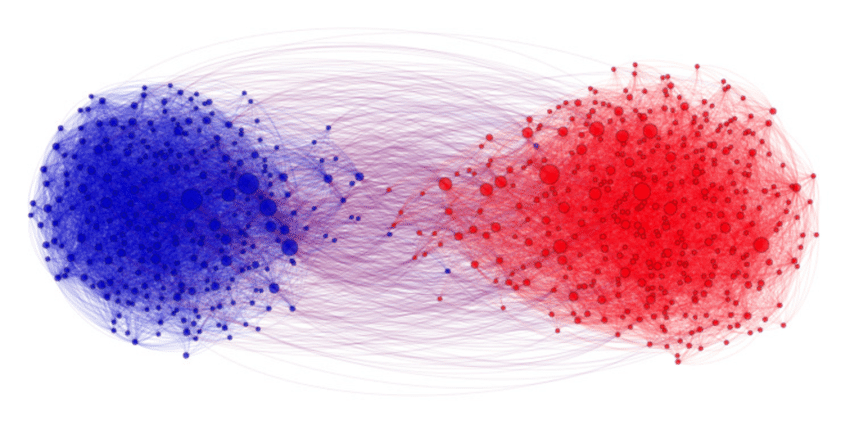
\includegraphics[width=\textwidth]{png/uvod.png}
    % add footnote
    \begin{tiny}
        Izvor: Interian, Ruben i Ribeiro, Celso. (2018). An empirical investigation of network polarization. Applied Mathematics and Computation. 339. 651-662. 10.1016/j.amc.2018.07.066.
    \end{tiny}
\end{frame}

\begin{frame}
	\frametitle{Ugrađivanje (embedovanje) čvorova}
	Neka je $ G = (V, E) $ graf, tada je ugrađivanje (embedovanje) funkcija 

	$$ U : V \to \mathbb{R}^n $$ 

	koja preslikava čvorove grafa u n-dimenzionalni euklidski prostor tako da čvorovi koji su dosta međusobno povezani budu blizu po euklidskom rastojanju
	

\end{frame}

\begin{frame}{node2vec algoritam}
	\centering
    \begin{tikzpicture}[node distance=2cm]

    % Blokovi
    \node (walks) [block] {Slučajne šetnje po čvorovima grafa};
    \node (embedding) [block, below of=walks] {Ugrađivanje (Embedding)};

    % Strelice
    \draw [arrow] (walks) -- (embedding);

    \end{tikzpicture}
\end{frame}

\begin{frame}{Ciljevi istraživanja}
    \begin{itemize}
        \item Implementacija paralelne verzije node2vec algoritma
        \item Evaluacija performansi na velikim realnim i sintetičkim mrežama sa različitim metodama particionisanja
        \item Poređenje kvaliteta dobijenog ugrađivanja sa serijskom verzijom
    \end{itemize}
\end{frame}


\section{Arhitektura}
\begin{frame}{Arhitektura}
    \centering
    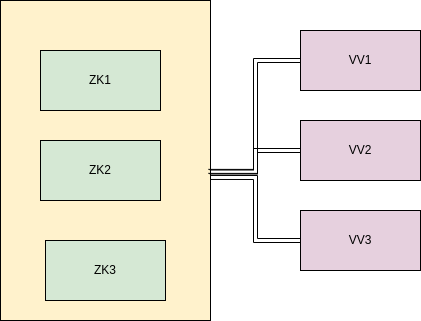
\includegraphics[height=0.8\textheight]{./png/Arhitektura i infrastruktura.drawio.png}
\end{frame}

\begin{frame}{Način rada - master i radni čvorovi}
    \begin{columns}
        \begin{column}{0.5\textwidth}
            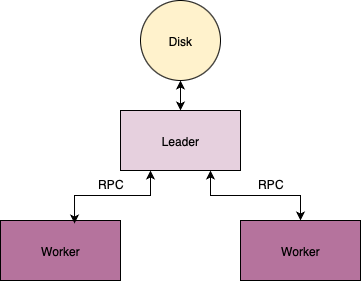
\includegraphics[height=0.5\textheight]{./png/Classic mode.drawio.png}
    \end{column}
    \begin{column}{0.5\textwidth}
        \begin{itemize}
            \item Master čvor:
            \begin{itemize}
                \item Učitava graf iz baze podataka
                \item Particioniše graf
                \item Raspoređuje particije po radnim čvorovima
                \item Prikuplja rezultate od radnih čvorova
                \item Spaja rezultate u konačno ugrađivanje
            \end{itemize}
            \item Radni čvorovi:
            \begin{itemize}
                \item Učitavaju particiju grafa iz baze podataka
                \item Izvršavaju node2vec algoritam na učitanom delu grafa
                \item Šalju rezultate nazad master čvoru
            \end{itemize}
        \end{itemize}
    \end{column}
    \end{columns}
\end{frame}

\begin{frame}{Način rada - Deljeni resursi}
    \begin{columns}
        \begin{column}{0.5\textwidth}
            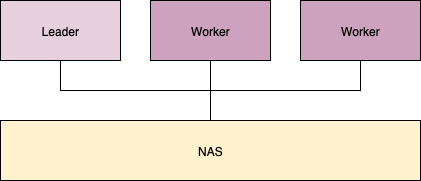
\includegraphics[width=0.5\textheight]{./png/NAS mode.drawio.png}
        \end{column}
        \begin{column}{0.5\textwidth}
            \begin{itemize}
                \item Izabere se jedan glavni čvor koji radi koordinaciju zadataka.
                \item Koordinator prosleđuje reference ka particijama
                \item Svi procesi imaju deljeno skladište za podatke
                \item Značajno pogodnije da se koristi sa integracijom sa SLURM-om.
            \end{itemize}
        \end{column}
    \end{columns}
\end{frame}

\section{Blokovski prikaz algoritma}
\begin{frame}{Blokovski prikaz algoritma}
    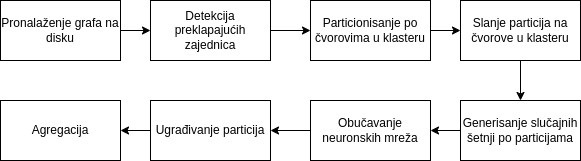
\includegraphics[width=\textwidth]{./png/Blokovski prikaz algoritma.drawio.png}
\end{frame}

\section{Particionisanje - LFM algoritam}
\begin{frame}{Detekcija preklapajućih zajednica}
    \begin{itemize}
        \item Algoritam za detekciju preklapajućih zajednica 
        \item Za svaki čvor koji nije dodeljen zajednici, dodeljuje se nova zajednica 
        \item Dodaju se susedni čvorovi čvorova u zajednici čije dodavanje uvećava kvalitet zajednice po funkciji $ f = \frac{k_\text{in}}{(k_\text{out} + k_\text{in})^\alpha} $ 
        \item Nakon dodavanja, uklanjaju se čvorovi čije uklanjanje povećava kvalitet zajednice
        \item Postupak se ponavlja sve dok postoje čvorovi koji nisu dodeljeni nekoj zajednici
    \end{itemize}
\end{frame}

\begin{frame}{Detekcija preklapajućih zajednica - modifikacija algoritma}
    \begin{itemize}
        \item Zbog povećanja brzine, algoritam se modifikuje tako da ne traje sve dok postoje čvorovi koji nisu dodeljeni zajednici
        \item Umesto toga, algoritam se izvršava dok određeni broj čvorova nije dodeljen zajednici
    \end{itemize}
\end{frame}

\begin{frame}{Particionisanje po čvorovima u klasteru}
    \begin{itemize}
        \item Nakon detekcije zajednica, potrebno je rasporediti zajednice po čvorovima u klasteru
        \item U ovom radu, korišćen je bin packing algoritam
        \item Algoritam raspoređuje zajednice po čvorovima, tako da čvorovi u klasteru budu što sličniji po svom opterećenju
        \item Opterećenje čvora K, kom su raspoređene zajednice $ S_K $, je $ \sum_{s \in S_K} |s| $
        \item Težine se zatim sortiraju u opadajućem redosledu, počevši od najveće.
        \item Inicijalno, maksimalna veličina (kapacitet) particije je prosečna veličina zajednice 
    \end{itemize}
\end{frame}

\begin{frame}
    \frametitle{Particionisanje po čvorovima u klasteru}
    \begin{itemize}
        \item Algoritam dodeljuje particije zajednicama, počevši od najveće zajednice. Uvek se dodeljuje particija koja je najmanje opterećena
        \item Ukoliko ne postoji particija koja ima potreban kapacitet, kapacitet particija se povećava za prosečnu veličinu zajednice koja još nije dodeljena particiji. 
        \item Ovaj proces se ponavlja dok sve zajednice ne budu raspoređene.
    \end{itemize}
\end{frame}


\begin{frame}
    \frametitle{Particionisanje - LPA algoritam}
    \begin{itemize}
        \item Algoritam zasnovan na širenju oznaka (Label Propagation Algorithm - LPA)
        \item Inicijalno, svaki čvor ima jedinstvenu oznaku
        \item U svakoj iteraciji, svaki čvor ažurira svoju oznaku na onu koja je najčešća među njegovim susedima
        \item Proces se ponavlja dok se oznake ne stabilizuju
        \item Nakon što su zajednice detektovane, koristi se isti bin packing algoritam za raspoređivanje zajednica po čvorovima u klasteru
    \end{itemize}
\end{frame}

\section{Gubici strukturnih informacija}
\begin{frame}{Mera gubitka strukturnih informacija}
    \begin{columns}
		\begin{column}{0.5\textwidth}
            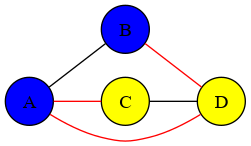
\includegraphics[width=\textwidth]{dot/graf.png}
		\end{column}
		\begin{column}{0.5\textwidth}
            Neka je $ E_p $ skup svih grana koje sadrže čvorove takve da su oba čvora u particiji $ p $  i neka je $ P $ skup svih particija za graf $ G = (V, E) $
            
            Tada je mera gubitka strukturnih informacija $ L $ definisana kao
            
            $$ L = 1-\frac{\sum_{p \in P} |E_p|}{|E|} $$
            
            , gde je $ |E_p| $ broj grana koje sadrže čvorove iz particije $ p $, a $ |E| $ ukupan broj grana u grafu $ G $.
		\end{column}
	\end{columns}
\end{frame}

\section{Korišćeni skupovi podataka}
\begin{frame}{Skupovi podataka}
    \begin{itemize}
        \item Poznati grafovi iz literature 
        \begin{itemize}
            \item Zaharijev karate klub
            \item Les Miserables
            \item Davis southern women
            \item Florentine families
        \end{itemize}
        \item CITESEER
        \item AstroPh
        \item Cit-HepPh
        \item Cit-HepTh
        \item Twitch 
        \item Sintetički grafovi generisani korišćenjem Stochastic Block Model (SBM)
    \end{itemize}
\end{frame}

\section{Rezultati}
\begin{frame}{Vreme particionisanja za realne mreže iz literature i Twitch}
    \centering
    \begin{table}
        \label{tab:4.2}
        \begin{tabular}{p{1.4in}p{1in}p{0.5in}p{0.5in}}
        Mreža & Vreme particionisanja (s)& Broj čvorova & Broj grana \\
        \hline
        Zaharijev karate klub & 0.001 & 34 & 78 \\
        Les Mis & 0.004 & 77 & 254 \\
        Davis southern women & 0.004 & 32 & 89 \\
        Florentine families & 0.0006 & 15 & 20 \\
        Twitch  & 1638.00 & 168114 & 6797557 \\
    \end{tabular}
\end{table}
\end{frame}
    
\begin{frame}{Vreme particionisanja za sintetički graf}
    \centering
    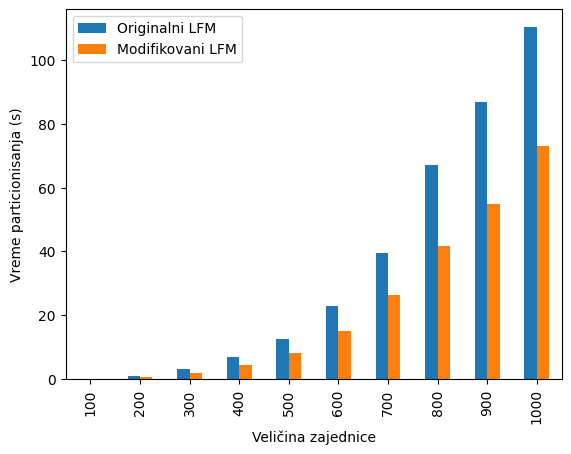
\includegraphics[height=0.8\textheight]{csv/4.3.png}
\end{frame}

\begin{frame}
    \frametitle{Ukupno vreme ugrađivanja na sintetičkom grafu}
    \centering
    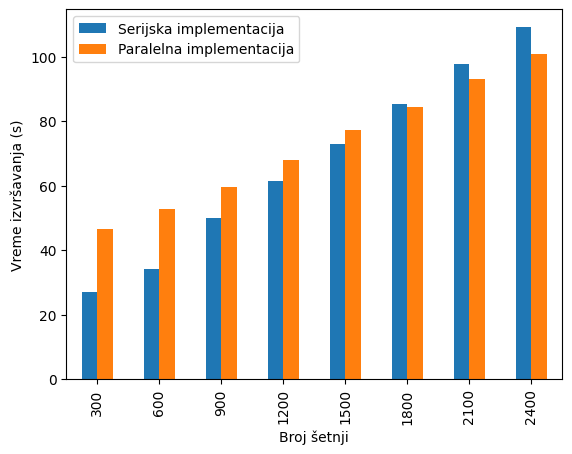
\includegraphics[height=0.8\textheight]{csv/4.13.png}
\end{frame}

\begin{frame}{Rezultati - vreme ugrađivanja na SBM sa 10M ivica}
    $$ \alpha = 1 \quad \text{Broj particija} = 16 $$
    \begin{table}
    \caption{Uporedna analiza performansi za LFM algoritam particionisanja}
    \label{tab:Performance_comparison_max_Node2Vec_vs_modified__lfm_on_SBM_10M_with_varying_threshold}
    \begin{tabular}{p{1in}p{1in}}
    \hline 
    Prag & Vreme particionisanja \\
    \hline
    0.000000 & 14118.587150 \\
    0.500000 & 12948.078974 \\
    1.000000 & 0.005604 \\
    \hline
    \end{tabular}
    \end{table}
    
\end{frame}

\begin{frame}
\begin{table}
\caption{Uporedna analiza performansi za LFM algoritam particionisanja}
\label{tab:Performance_comparison_max_Node2Vec_vs_modified__lfm_on_SBM_10M_with_varying_alpha}
\begin{tabular}{p{1in}p{1in}p{1in}}
\hline
$\alpha$  & Vreme particionisanja & Vreme ugrađivanja na 16 čvorova \\
\hline
1.000000 & 15151.445818 & 96.892017 \\
1.500000 & 14384.355827 & 83.339856 \\
2.000000 & 1489.028646 & 60.098522 \\
\hline
\end{tabular}
\end{table}
    
\end{frame}

\begin{frame}
\begin{table}
    
\caption{Uporedna analiza performansi za LFM algoritam particionisanja}
\label{tab:Performance_comparison_max_Node2Vec_vs_lfm_on_SBM_10M_with_varying_partition_num}
\begin{tabular}{p{1in}p{1in}p{1in}p{1in}}
\hline
 & Vreme particionisanja & Paralelna implementacija \\
Broj particija &  &  &  \\
\hline
1 & 77.875600 & 107.061880  \\
2 & 155.384691 & 102.909459 \\
4 & 318.065973 & 90.397061 \\
8 & 604.270801 & 107.493993 \\
16 & 1202.096511 & 113.680622 \\
32 & 2384.997995 & 122.427380 \\
\hline
\end{tabular}
\end{table}
\end{frame}

\begin{frame}{Balance i Edge Cut poređenje: LPA vs. LFM}
\begin{table}[h]
\centering
\begin{tabular}{lcccc}
\hline
\textbf{Network} & \textbf{Balance (LPA)} & \textbf{Edge cut (LPA)} & \textbf{Balance (LFM)} & \textbf{Edge cut (LFM)} \\
\hline
CITESEER   & 0.000612 & 22\%    & 0.0016  & 68.8\%  \\
AstroPh    & 0.824    & 8.4\%   & 0.00085 & 74.5\%  \\
Cit-HepPh  & 0.00005  & 20.6\%  & 0.00147 & 73.8\%  \\
Cit-HepTh  & 0.483    & 11.74\% & 0.0023  & 74.14\% \\
\hline
\end{tabular}
\caption*{Balance and edge cut for label propagation and modified LFM partitioning on real-world networks.}
\end{table}
\end{frame}


\begin{frame}{F1 ocene za LFM threshold = 0, $\alpha = 1$}
\begin{table}[h]
\centering
\begin{tabular}{lccc}
\hline
\textbf{Network} & \textbf{Dim} & \textbf{F1 sequential} & \textbf{F1 on 2 nodes} \\
\hline
CITESEER   & 50  & 24\%  & 33\% \\
AstroPh    & 100 & 5.1\% & 6.6\% \\
Cit-HepPh  & 100 & 2.5\% & 2.8\% \\
Cit-HepTh  & 100 & 2.9\% & 3.2\% \\
\hline
\end{tabular}
\caption*{F1 scores for Node2Vec with modified LFM partitioning.}
\end{table}
\end{frame}

\begin{frame}{F1 ocene za 4 particije (threshold = 0)}
\begin{table}[h]
\centering
\begin{tabular}{lc}
\hline
\textbf{Network} & \textbf{F1 score on 4 nodes} \\
\hline
CITESEER   & 18.99\% \\
AstroPh    & 8.97\%  \\
Cit-HepPh  & 3.43\%  \\
Cit-HepTh  & 4.33\%  \\
\hline
\end{tabular}
\caption*{F1 scores for distributed Node2Vec with modified LFM partitioning (4 partitions).}
\end{table}
\end{frame}

\begin{frame}{F1 ocene za 4 particije (threshold = 0.5)}
Table 9: F1 scores when 50\% unassigned vertices threshold is used.
\begin{table}[h]
\centering
\begin{tabular}{lc}
\hline
\textbf{Network} & \textbf{F1 score on 4 nodes} \\
\hline
CITESEER   & 28.46\% \\
AstroPh    & 9.21\%  \\
Cit-HepPh  & 3.37\%  \\
Cit-HepTh  & 4.30\%  \\
\hline
\end{tabular}
\caption*{F1 scores for Node2Vec with LFM partitioning (threshold 50\%).}
\end{table}
\end{frame}

\begin{frame}{F1 ocene za slučajno particionisanje (threshold = 1)}
\begin{table}[h]
\centering
\begin{tabular}{lc}
\hline
\textbf{Network} & \textbf{F1 score on 4 nodes} \\
\hline
CITESEER   & 26.67\% \\
AstroPh    & 8.23\%  \\
Cit-HepPh  & 3.08\%  \\
Cit-HepTh  & 3.76\%  \\
\hline
\end{tabular}
\caption*{F1 scores for random partitioning (equal probability).}
\end{table}
\end{frame}

\begin{frame}{F1 ocene za Label Propagation particionisanje}
\begin{table}[h]
\centering
\begin{tabular}{lc}
\hline
\textbf{Network} & \textbf{F1 score on 4 nodes} \\
\hline
CITESEER   & 44.34\% \\
AstroPh    & 19.48\% \\
Cit-HepPh  & 4.8\%   \\
Cit-HepTh  & 5.1\%   \\
\hline
\end{tabular}
\caption*{F1 scores for distributed Node2Vec with label propagation partitioning.}
\end{table}
\end{frame}

\begin{frame}{Zaključak}
\begin{itemize}
  \item Eksperimentalni rezultati pokazuju da predloženi sistem efikasno čuva strukturu zajednica unutar particija, što dovodi do visokokvalitetnih ugrađivanja koja dobro hvataju odnose između čvorova u originalnom grafu.
  \item Modifikovani LFM algoritam sa kriterijumom ranog zaustavljanja značajno smanjuje vreme particionisanja, a pritom zadržava kvalitet particija.
  \item \emph{Label propagation} pokazuje potencijal u generisanju uravnoteženih particija sa manjim presekom grana (edge cut), što dodatno poboljšava kvalitet urezivanja.
\end{itemize}
\end{frame}




\begin{frame}
	\begin{center}
		\Huge Hvala na pažnji!
	\end{center}
\end{frame}


\end{document}
